% !TeX document-id = {fb8a2ef5-cdaf-49da-b79d-0a8152e677cd}
% !TeX TS-program = XeLaTeX
\documentclass[a4paper,12pt]{report}

% polyglossia should go first!
\usepackage{polyglossia} % multi-language support
\setmainlanguage{russian}
\setotherlanguage{english}

\usepackage{amsmath} % math symbols, new environments and stuff
\usepackage{unicode-math} % for changing math font and unicode symbols
\usepackage[style=english]{csquotes} % fancy quoting
\usepackage{microtype} % for better font rendering
\usepackage{hyperref} % for refs and URLs
\usepackage{graphicx} % for images (and title page)
\usepackage{geometry} % for margins in title page
\usepackage{tabu} % for tabulars (and title page)
\usepackage[section]{placeins} % for float barriers
\usepackage{titlesec} % for section break hooks
\usepackage{listings} % for listings 
\usepackage{upquote} % for good-looking quotes in source code (used for custom languages)
\usepackage{xcolor} % colors!
\usepackage{enumitem} % for unboxed description labels (long ones)
\usepackage{caption}
\usepackage{multirow}
\usepackage{varwidth}
\usepackage{longtable}

\defaultfontfeatures{Mapping=tex-text} % for converting "--" and "---"
\setmainfont{CMU Serif}
\setsansfont{CMU Sans Serif}
\setmonofont{CMU Typewriter Text}
\setmathfont{XITS Math}
\MakeOuterQuote{"} % enable auto-quotation

% new page and barrier after section, also phantom section after clearpage for
% hyperref to get right page.
% clearpage also outputs all active floats:
\newcommand{\sectionbreak}{\phantomsection}
\newcommand{\subsectionbreak}{\FloatBarrier}
\renewcommand{\thesection}{\arabic{section}} % no chapters
\numberwithin{equation}{section}
%\usetikzlibrary{shapes,arrows,trees}

\newcommand{\itemtt}[1][]{\item[\texttt{#1}:]} % tt-ed items (for protocol descriptions)

\definecolor{bluekeywords}{rgb}{0.13,0.13,1}
\definecolor{greencomments}{rgb}{0,0.5,0}
\definecolor{turqusnumbers}{rgb}{0.17,0.57,0.69}
\definecolor{redstrings}{rgb}{0.5,0,0}
\setmonofont{Consolas} %to be used with XeLaTeX or LuaLaTeX
\definecolor{bluekeywords}{rgb}{0,0,1}
\definecolor{greencomments}{rgb}{0,0.5,0}
\definecolor{redstrings}{rgb}{0.64,0.08,0.08}
\definecolor{xmlcomments}{rgb}{0.5,0.5,0.5}
\definecolor{types}{rgb}{0.17,0.57,0.68}

\lstloadlanguages{bash, python, Java}

\lstset{
  frame=none,
  xleftmargin=2pt,
  stepnumber=1,
  numbers=left,
  numbersep=5pt,
  numberstyle=\ttfamily\tiny\color[gray]{0.3},
  belowcaptionskip=\bigskipamount,
  captionpos=b,
  escapeinside={*'}{'*},
  language=python,
  tabsize=2,
  emphstyle={\bf},
  commentstyle=\it,
  stringstyle=\mdseries\rmfamily,
  showspaces=false,
  keywordstyle=\bfseries\rmfamily,
  columns=flexible,
  basicstyle=\small\sffamily,
  showstringspaces=false,
  morecomment=[l]\%,
  breaklines=true,
  showlines=true
}
\renewcommand\lstlistingname{Листинг}

\date{\today}

\makeatletter
\let\thetitle\@title
\let\theauthor\@author
\let\thedate\@date
\makeatother

\makeatletter
\AtBeginDocument{%
    \expandafter\renewcommand\expandafter\subsection\expandafter{%
        \expandafter\@fb@secFB\subsection
    }%
}
\makeatother

\newcommand\LongMultirow[2]{%
  \multirow{#1}*{%
    \begin{varwidth}{5em}% --- or minipage, if you prefer a fixed width
    \flushright #2%
    \end{varwidth}}}

\begin{document}

\tableofcontents

\clearpage
\section*{Глоссарий}
\begin{itemize}
  \item комплекс
  \item сус
  \item сбн
  \item су  
  \item 
  \item задача
  \item пользователь
  \item вычислительный узел
  \item 
  \item x?
  \item 
  \item 
\end{itemize}

\clearpage
\section*{Введение}

\clearpage
\section{Аналитический раздел}
\subsection{Введение}
В данном разделе выполняется анализ предметной области.
Результаты анализа представляются в виде диаграм прецедентов и деятельности.

\subsection{Возможные прецеденты}
Комплекс при его работе предоставляет пользователю следующие варианты использования:
\begin{itemize}
  \item регистрация пользователя;
  \item авторизация пользователя;
  \item постановка задачи на исполнение;
  \item просмотр статуса задачи;
  \item отмена задачи.
\end{itemize}

Диаграмма этих и дополнительных служебных прецедентов приведена на рис.~\ref{fig:prec-common}.

\begin{figure}[b]
  \centering
  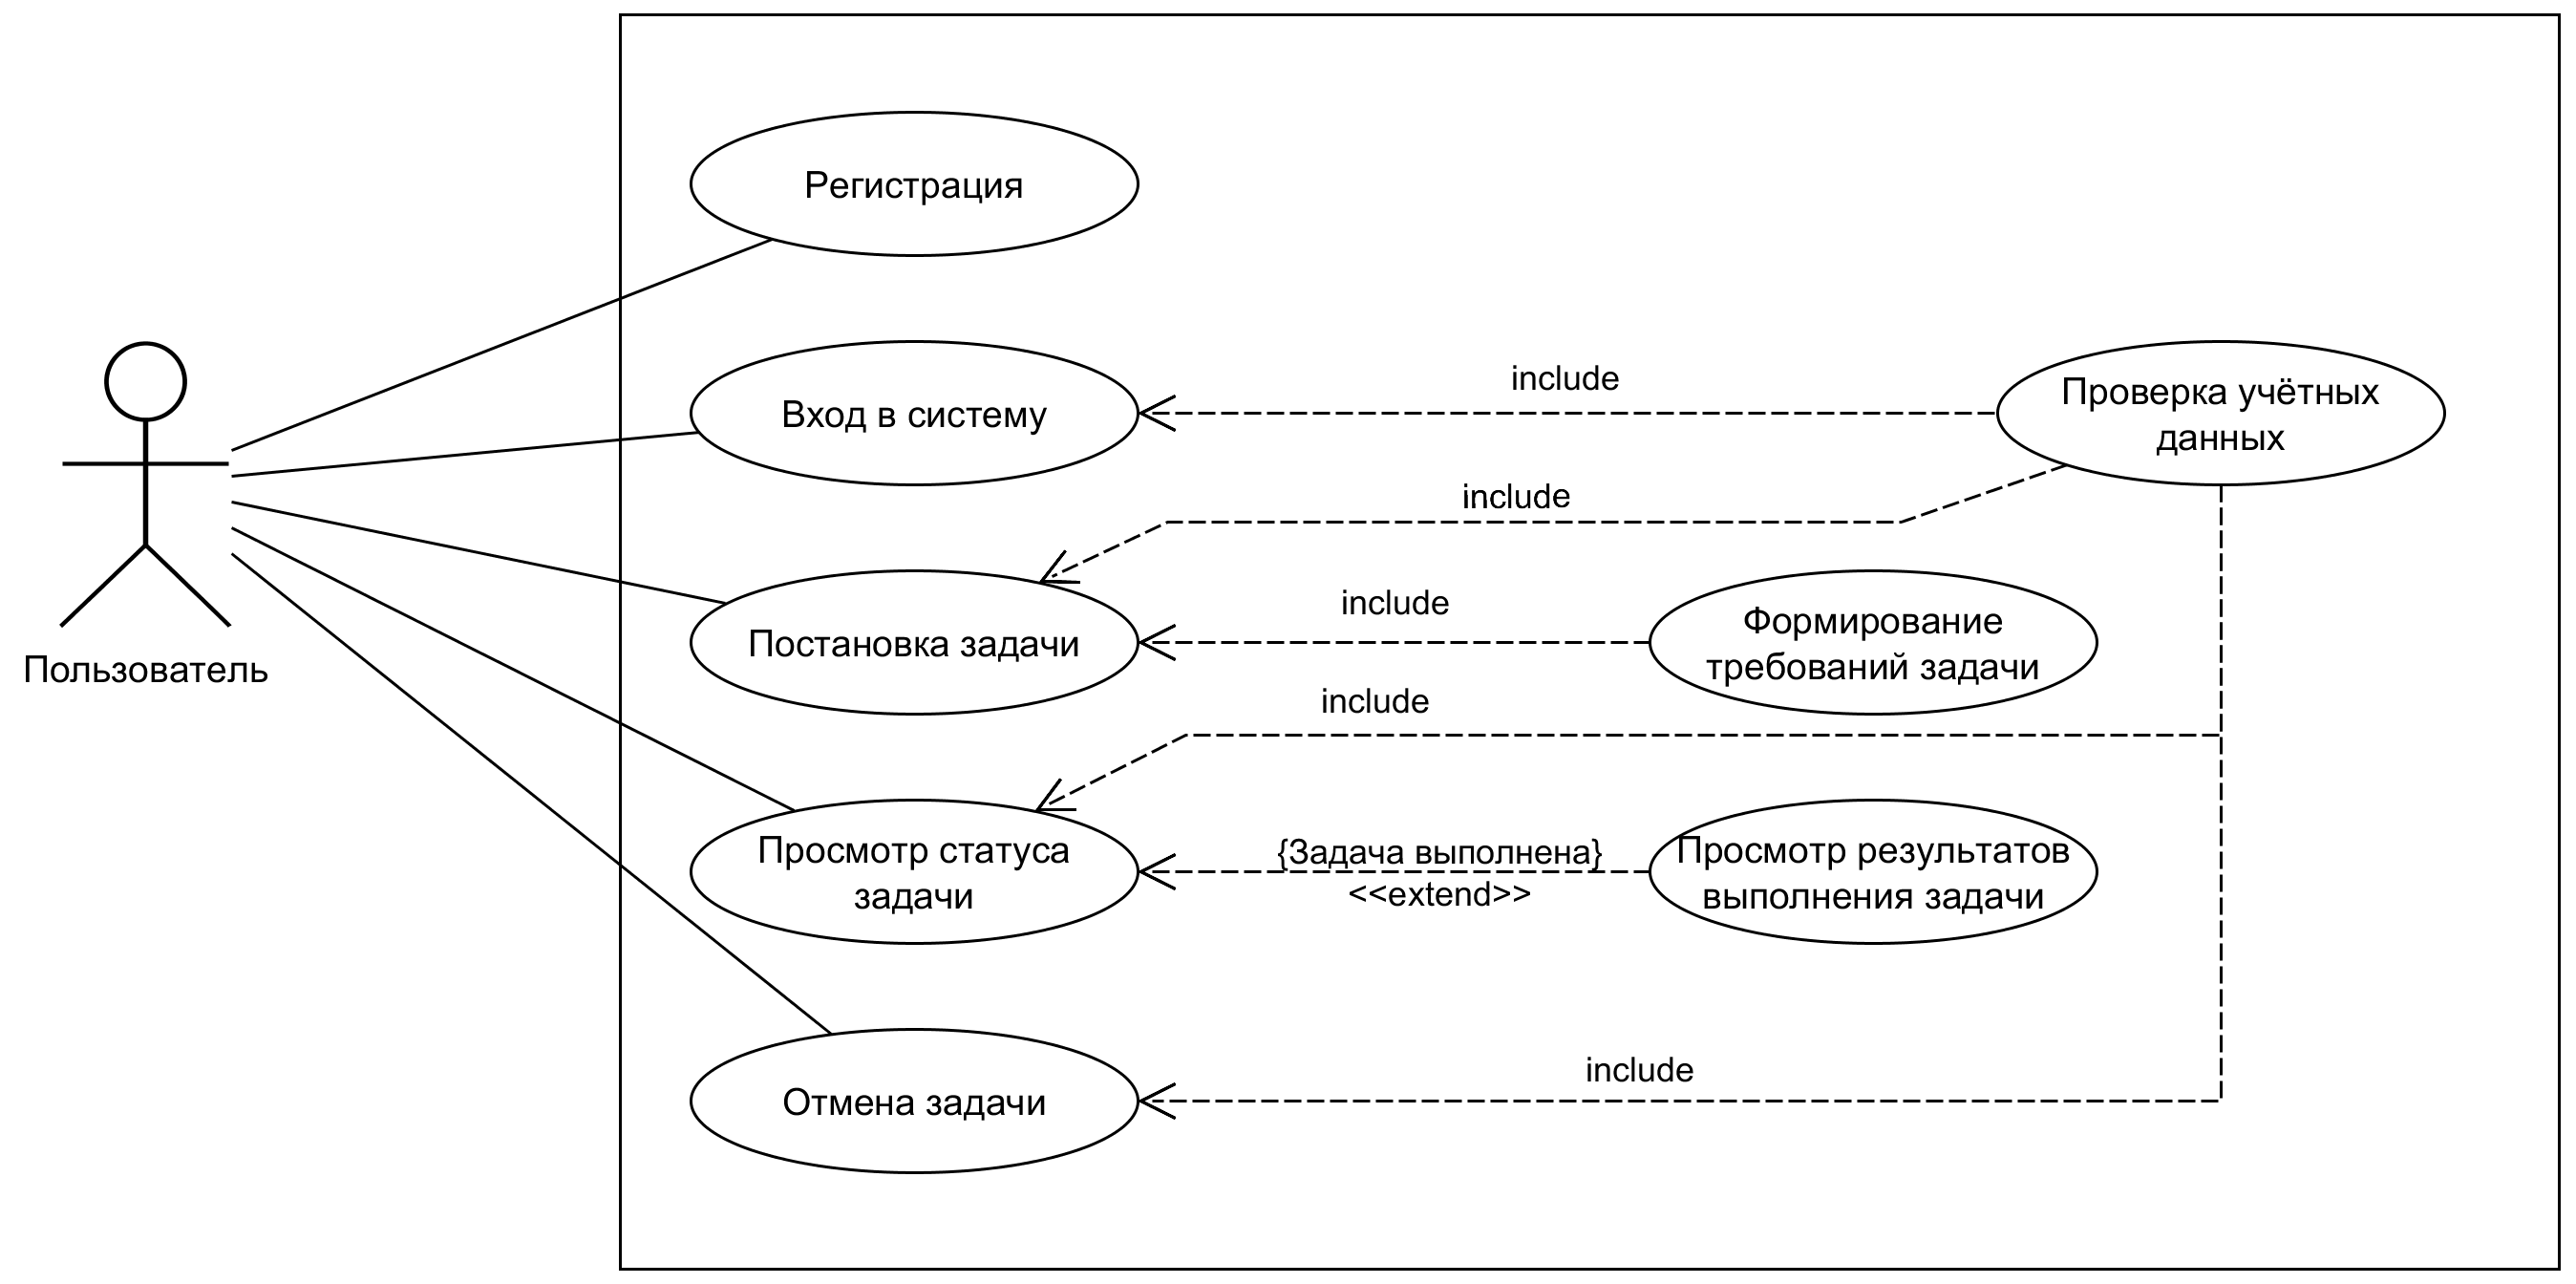
\includegraphics[width=.9\linewidth]{diagrams/common/usecase}
  \caption{Диаграмма прецедентов всего комплекса в целом}
  \label{fig:prec-common}
\end{figure}

С учётом требований к разделению внутреннего функционала комплекса, диаграмма прецедентов на рис.~\ref{fig:prec-common}
расщепляется на набор диаграмм, соответствующих каждой из выделенных подсистем.
Соответствующие диаграммы приведены на рисунках~\ref{fig:prec-session},\ref{fig:prec-logic},\ref{fig:prec-balancer}.

\begin{figure}
  \centering
  \begin{minipage}{.49\linewidth}
    \centering
    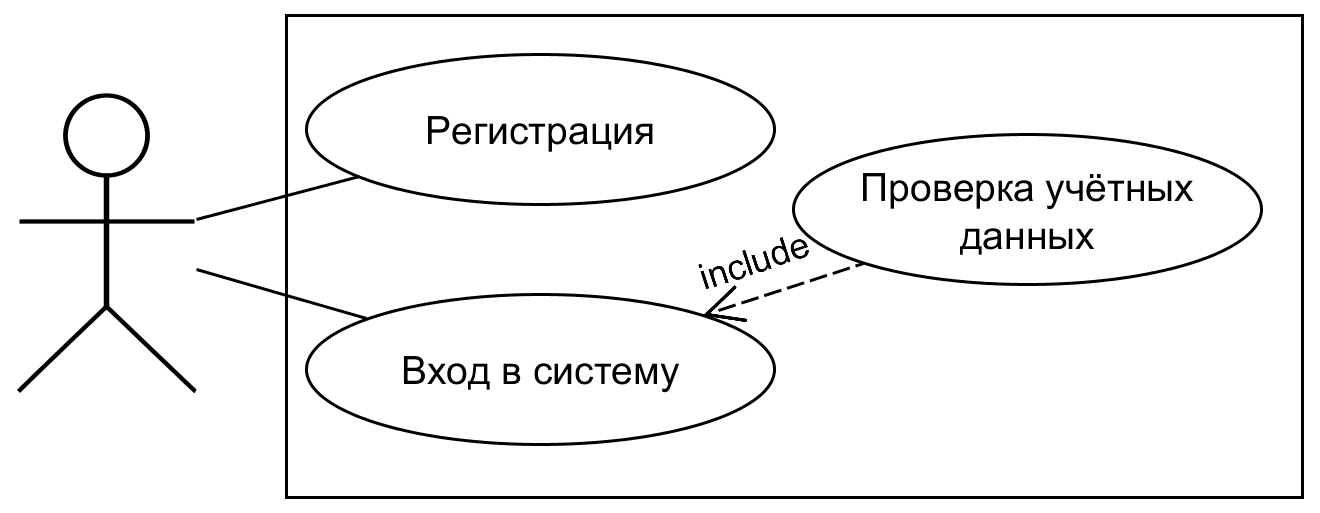
\includegraphics[width=\linewidth]{diagrams/session/usecase}
    \caption{Диаграмма прецедентов СУС}
    \label{fig:prec-session}
  \end{minipage}
  \hfill
  \begin{minipage}{.49\linewidth}
    \centering
    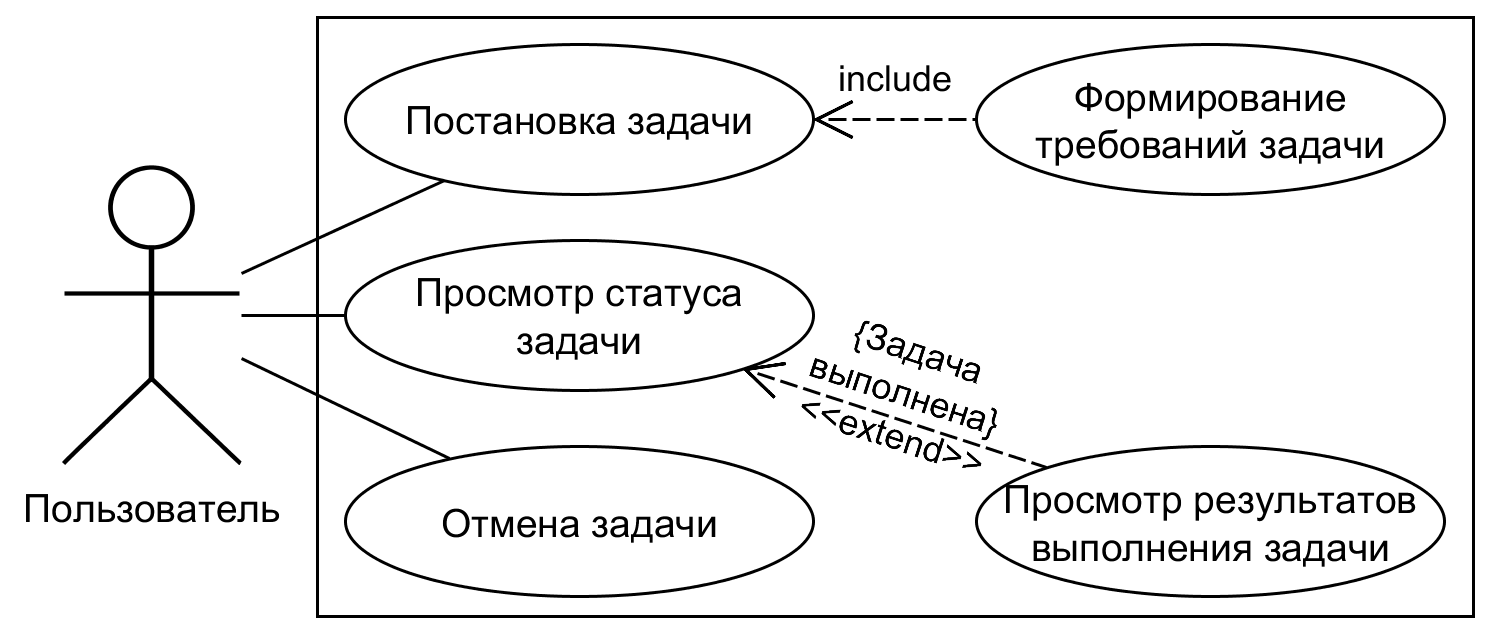
\includegraphics[width=\linewidth]{diagrams/logic/usecase}
    \caption{Диаграмма прецедентов СУ}
    \label{fig:prec-logic}
  \end{minipage}  
\end{figure}

\begin{figure}
  \centering
  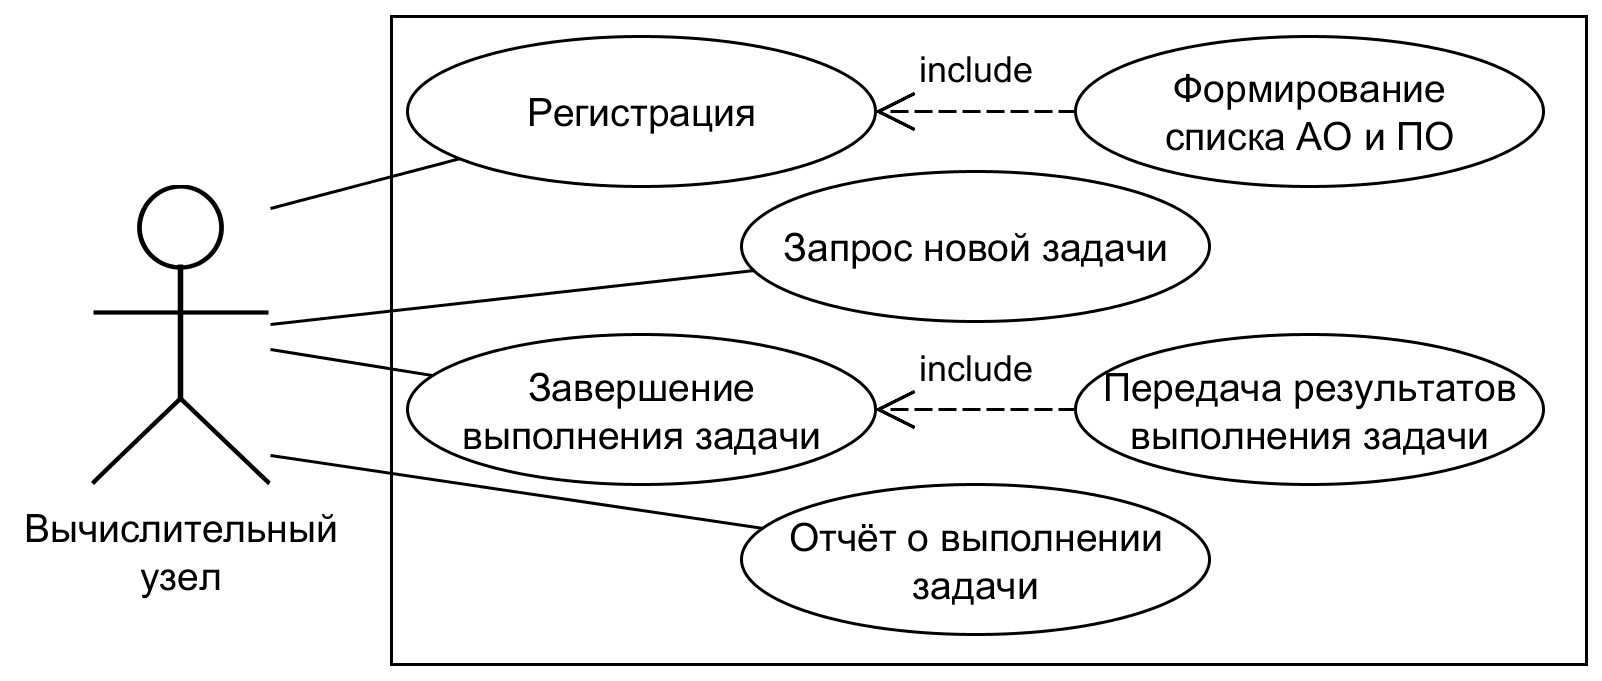
\includegraphics[width=.6\linewidth]{diagrams/balancer/usecase}
  \caption{Диаграмма прецедентов СБН}
  \label{fig:prec-balancer}
\end{figure}

\subsection{Осуществляемая деятельность}
Прецеденты, описанные в предыдущем пункте, отвечают определённой деятельности.
Диаграмма деятельности на рис.~\ref{fig:act-common} описывает полный процесс взаимодействия пользователя с комплексом.

С учётом требований к разделению внутреннего функционала комплекса, диаграмма деятельности на рис.~\ref{fig:act-common}
расщепляется на набор диаграмм, соответствующих определённым подсистемам из выделенных.

Диаграммы действий прецедентов подсистемы управления сессией "регистрация" и "вход в систему" приведены на рисунках~\ref{fig:act-register} и~\ref{fig:act-auth} соответственно.

Диаграммы действий прецедентов системы балансировки нагрузки "регистрация", "запрос новой задачи" и "завершение выполнения задачи" приведены на рисунках~\ref{fig:bal-register},~\ref{fig:bal-request} и~\ref{fig:bal-submit} соответственно.

Диаграммы действий прецедентов системы управления "постановка задачи" и "просмотр статсуа задачи" приведены на рисунках~\ref{fig:logic-place} и~\ref{fig:logic-view} соответственно.

\begin{figure}[h]
  \centering
  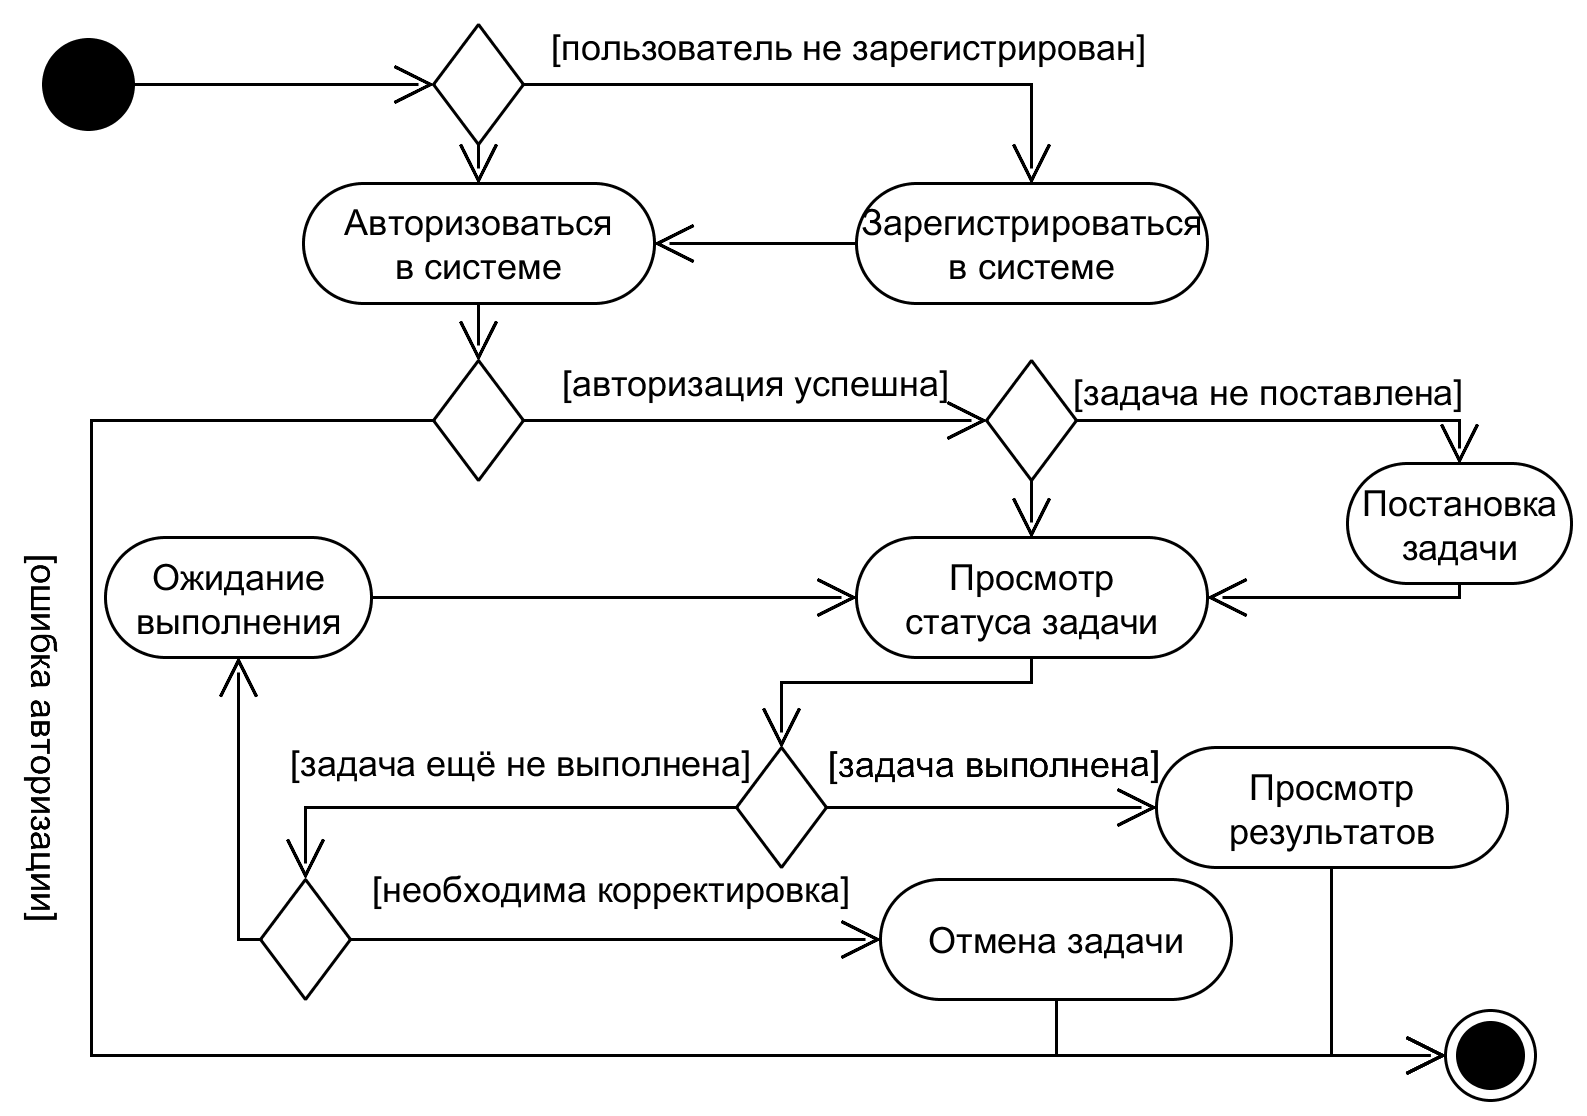
\includegraphics[width=.9\linewidth]{diagrams/common/activity}
  \caption{Диаграмма действий прецедента "общая деятельность" для системы в целом}
  \label{fig:act-common}
\end{figure}

\begin{figure}
  \centering
  \begin{minipage}{.43\linewidth}
    \centering
    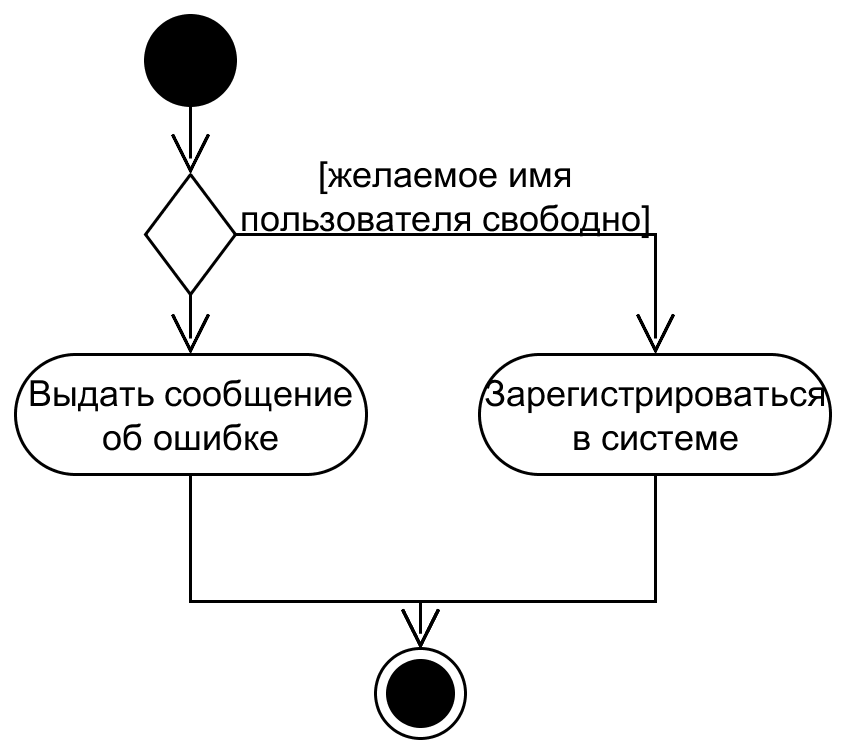
\includegraphics[width=\linewidth]{diagrams/session/activity-register}
    \caption{Диаграмма действий прецедента "регистрация" СУС}
    \label{fig:act-register}
  \end{minipage}
  \hfill
  \begin{minipage}{.53\linewidth}
    \centering
    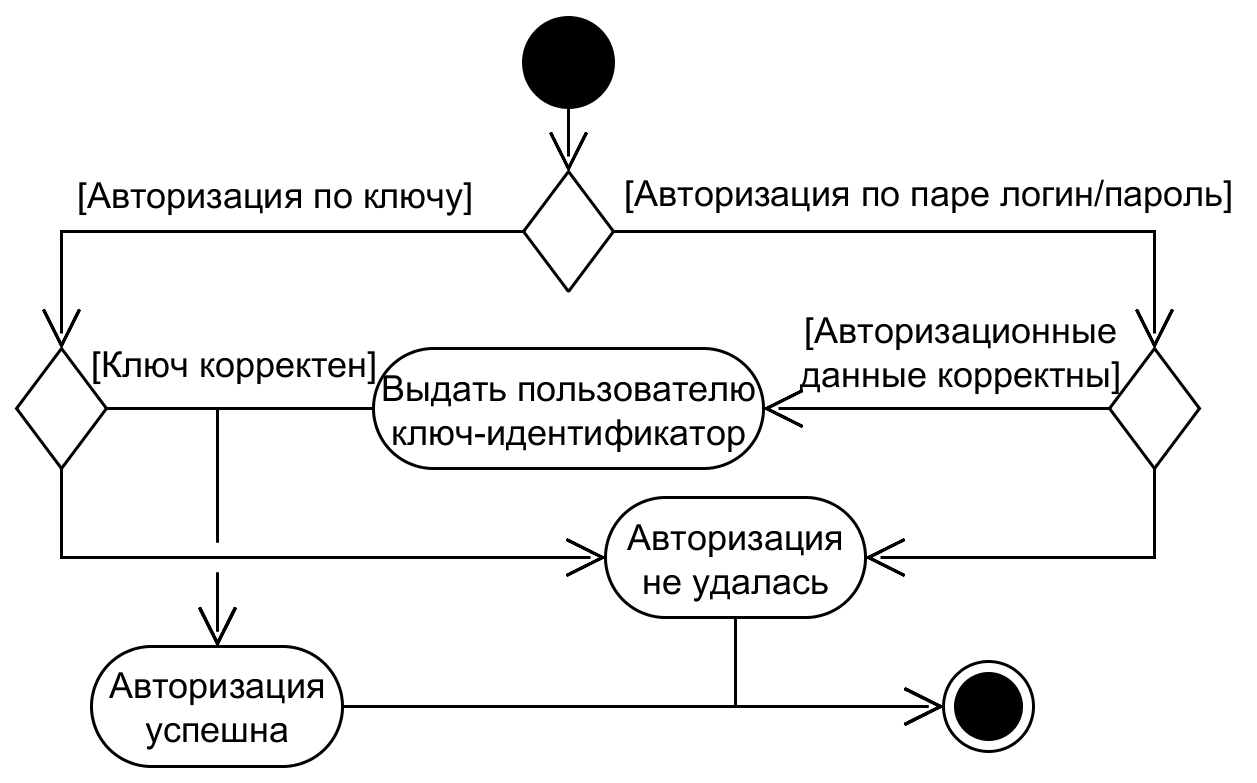
\includegraphics[width=\linewidth]{diagrams/session/activity-authorize}
    \caption{Диаграмма действий прецедента "вход в систему" СУС}
    \label{fig:act-auth}
  \end{minipage}  
\end{figure}

\begin{figure}  
  \centering
  \begin{minipage}{.49\linewidth}
    \centering
    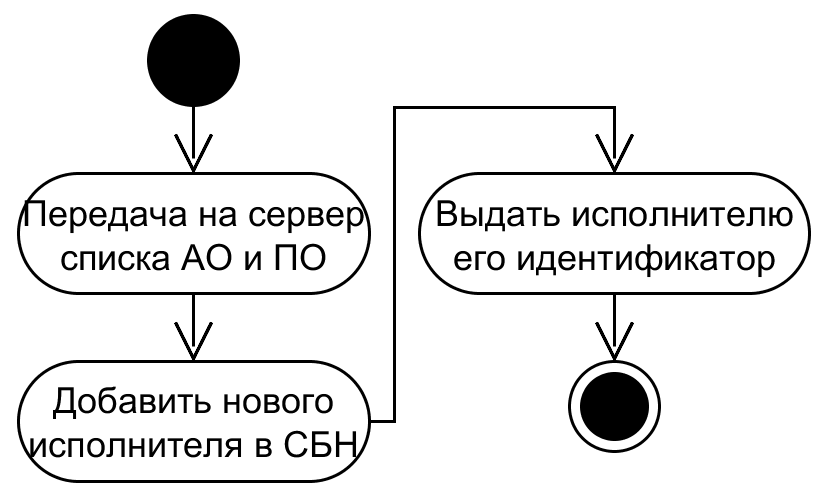
\includegraphics[width=\linewidth]{diagrams/balancer/activity-register}
    \caption{Диаграмма действий прецедента "регистрация" СБН}
    \label{fig:bal-register}
  \end{minipage}
  \hfill
  \begin{minipage}{.49\linewidth}
    \centering
    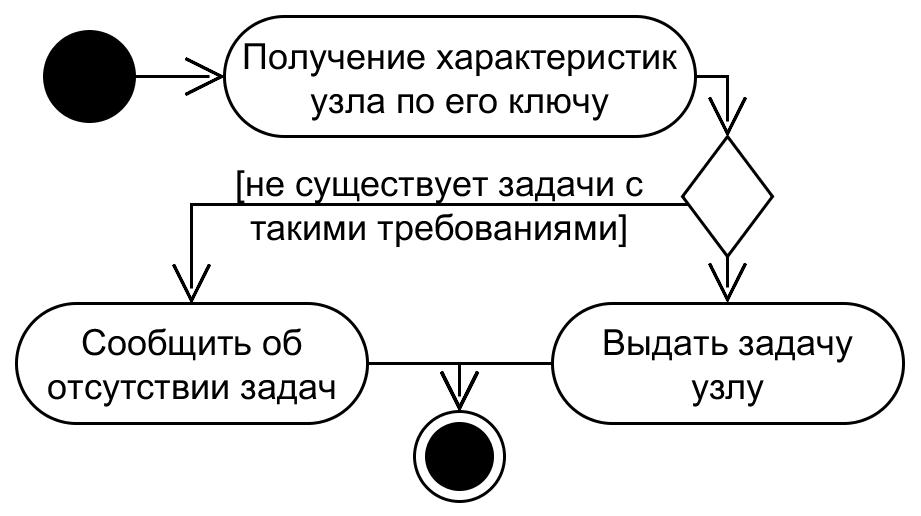
\includegraphics[width=\linewidth]{diagrams/balancer/activity-request}
    \caption{Диаграмма действий прецедента "запрос новой задачи" СБН}
    \label{fig:bal-request}
  \end{minipage}  
\end{figure}

\begin{figure}  
  \centering
  \begin{minipage}{.49\linewidth}
    \centering
    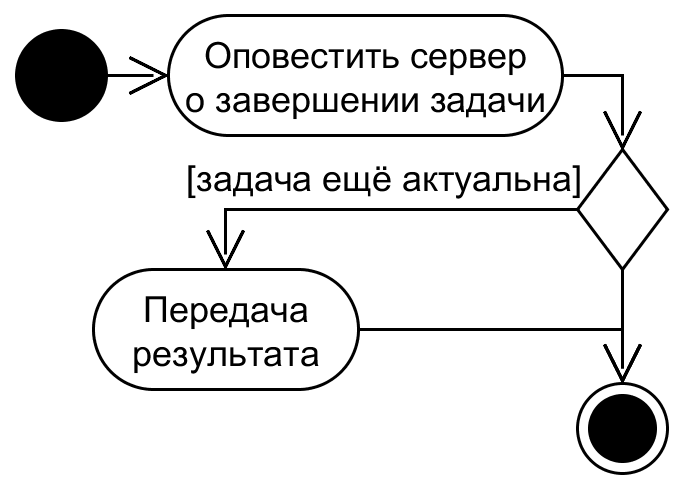
\includegraphics[width=\linewidth]{diagrams/balancer/activity-submit}
    \caption{Диаграмма действий прецедента "завершение выполнения задачи" СБН}
    \label{fig:bal-submit}
  \end{minipage} 
  \hfill
  \begin{minipage}{.49\linewidth}
    \centering
    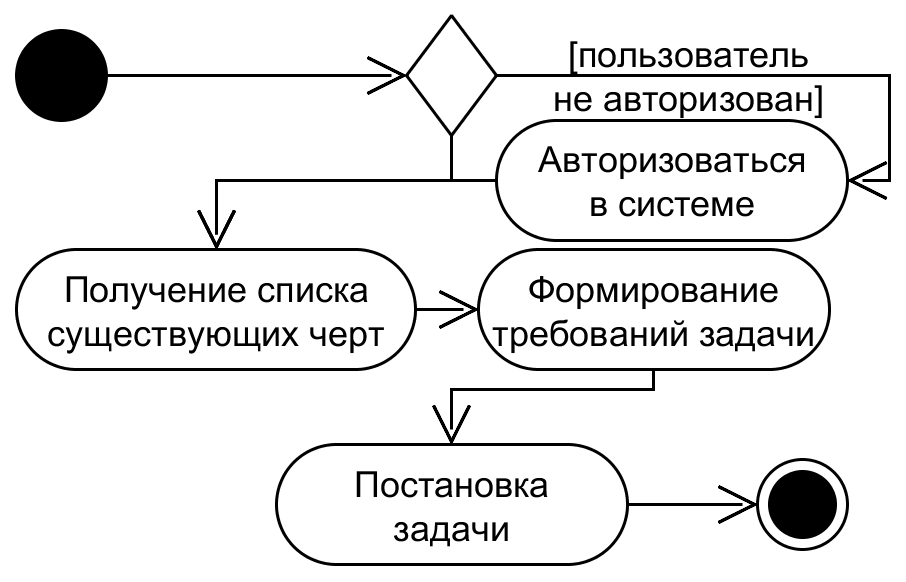
\includegraphics[width=\linewidth]{diagrams/logic/activity-place}
    \caption{Диаграмма действий прецедента "постановка задачи" СУ}
    \label{fig:logic-place}
  \end{minipage} 
\end{figure}

\begin{figure}
  \centering
  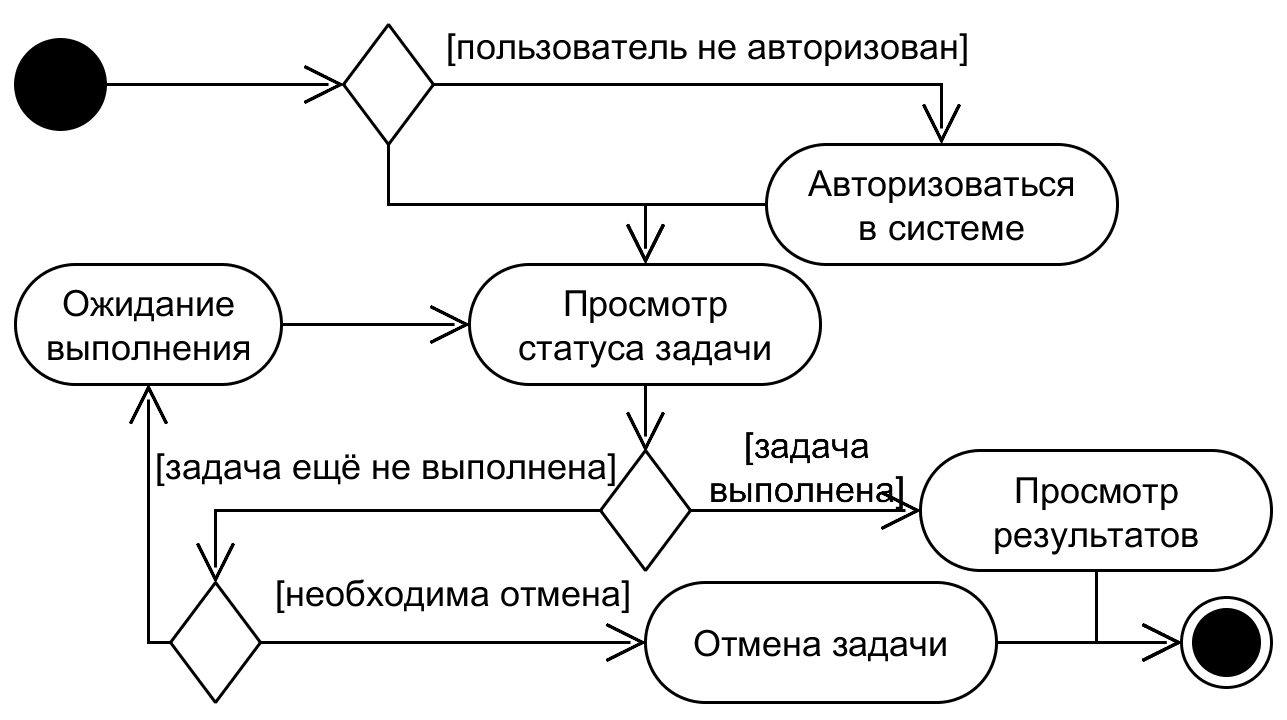
\includegraphics[width=\linewidth]{diagrams/logic/activity-view}
  \caption{Диаграмма действий прецедента "просмотр статсуа задачи" СУ}
  \label{fig:logic-view}
\end{figure}

\subsection{Вывод}
В данном разделе были приведены диаграммы, описывающие функционал основных узлов системы.
Данный анализ в дальнейшем используется для более строгой формализации функционала подсистем.

\clearpage
\section{Конструкторский раздел}
\subsection{Введение}
В данном разделе приводятся результаты проектирования системы.
С применением UML-диаграмм описывается общая структура комплекса и требуемый функционал отдельных узлов системы.

\subsection{Общая структура системы}
Для того, чтобы удовлетворить требованиям по предоставлению механизма деградации функциональности,
а также для упрощения процесса разработки, комплекс должен быть разделен на отдельные слабосвязанные элементы.

Различные подсистемы комплекса имеют некую модель поведения.
Поведение подсистемы описывается её активной и пассивной частью.
Активная часть соответствует действиям, которые подсистема выполняет разово либо с некоторой периодичностью, в автоматическом режиме.
Пассивная часть соответствует API подсистемы.
Взаимосвязи между различными компонентами системы приведены на диаграмме компонентов на рис.~\ref{fig:comp-common}.
Физическое размещение компонент по отдельным узлам проиллюстрировано на диаграмме развёртывания на рис.~\ref{fig:depl-common}.

\begin{figure}[b]
  \centering
  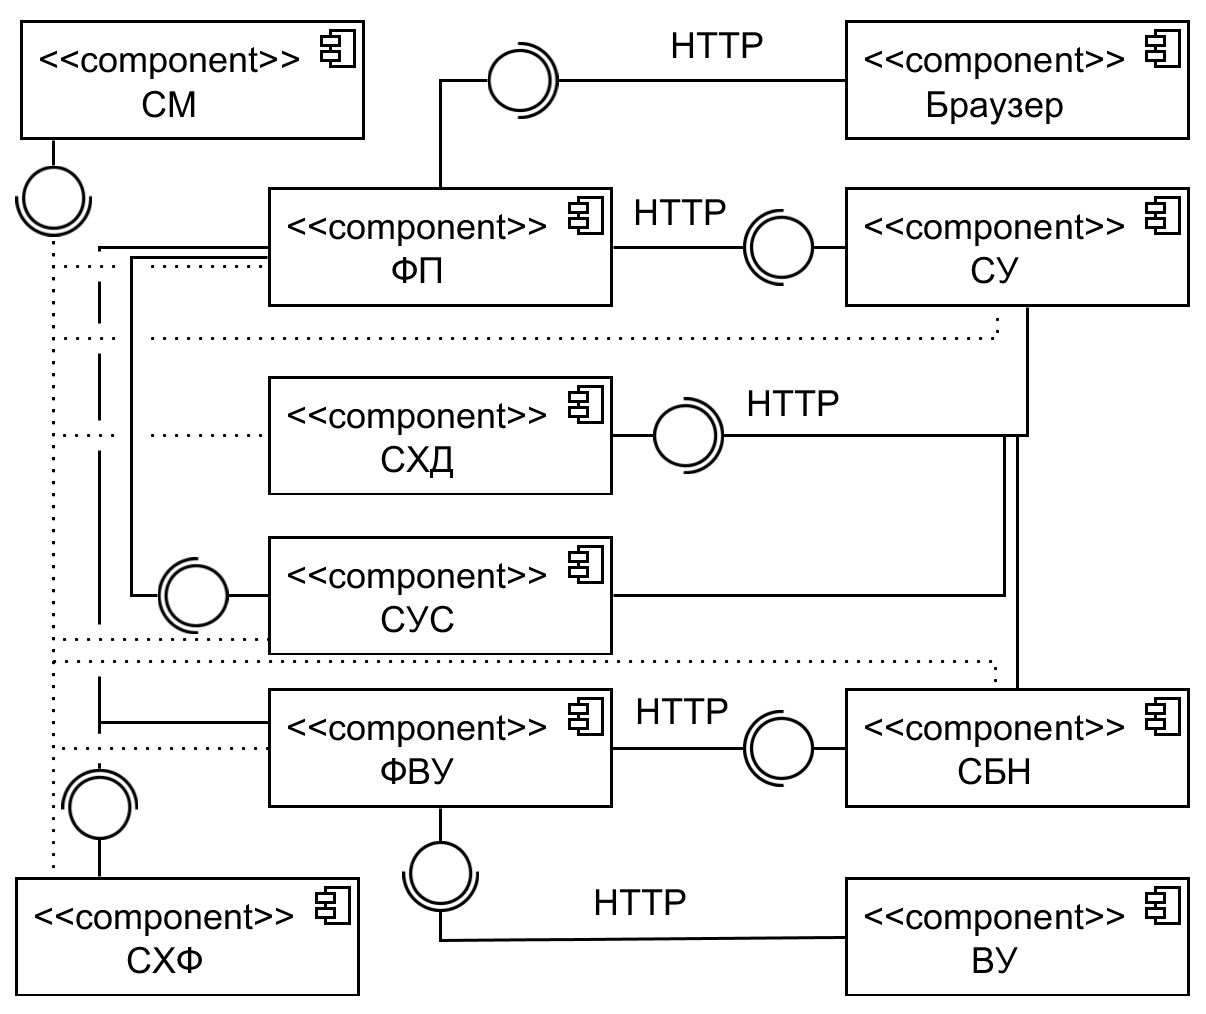
\includegraphics[width=.7\linewidth]{diagrams/common/component}
  \caption{Диаграмма компонент комплекса}
  \label{fig:comp-common}
\end{figure}

\begin{figure}
  \centering
  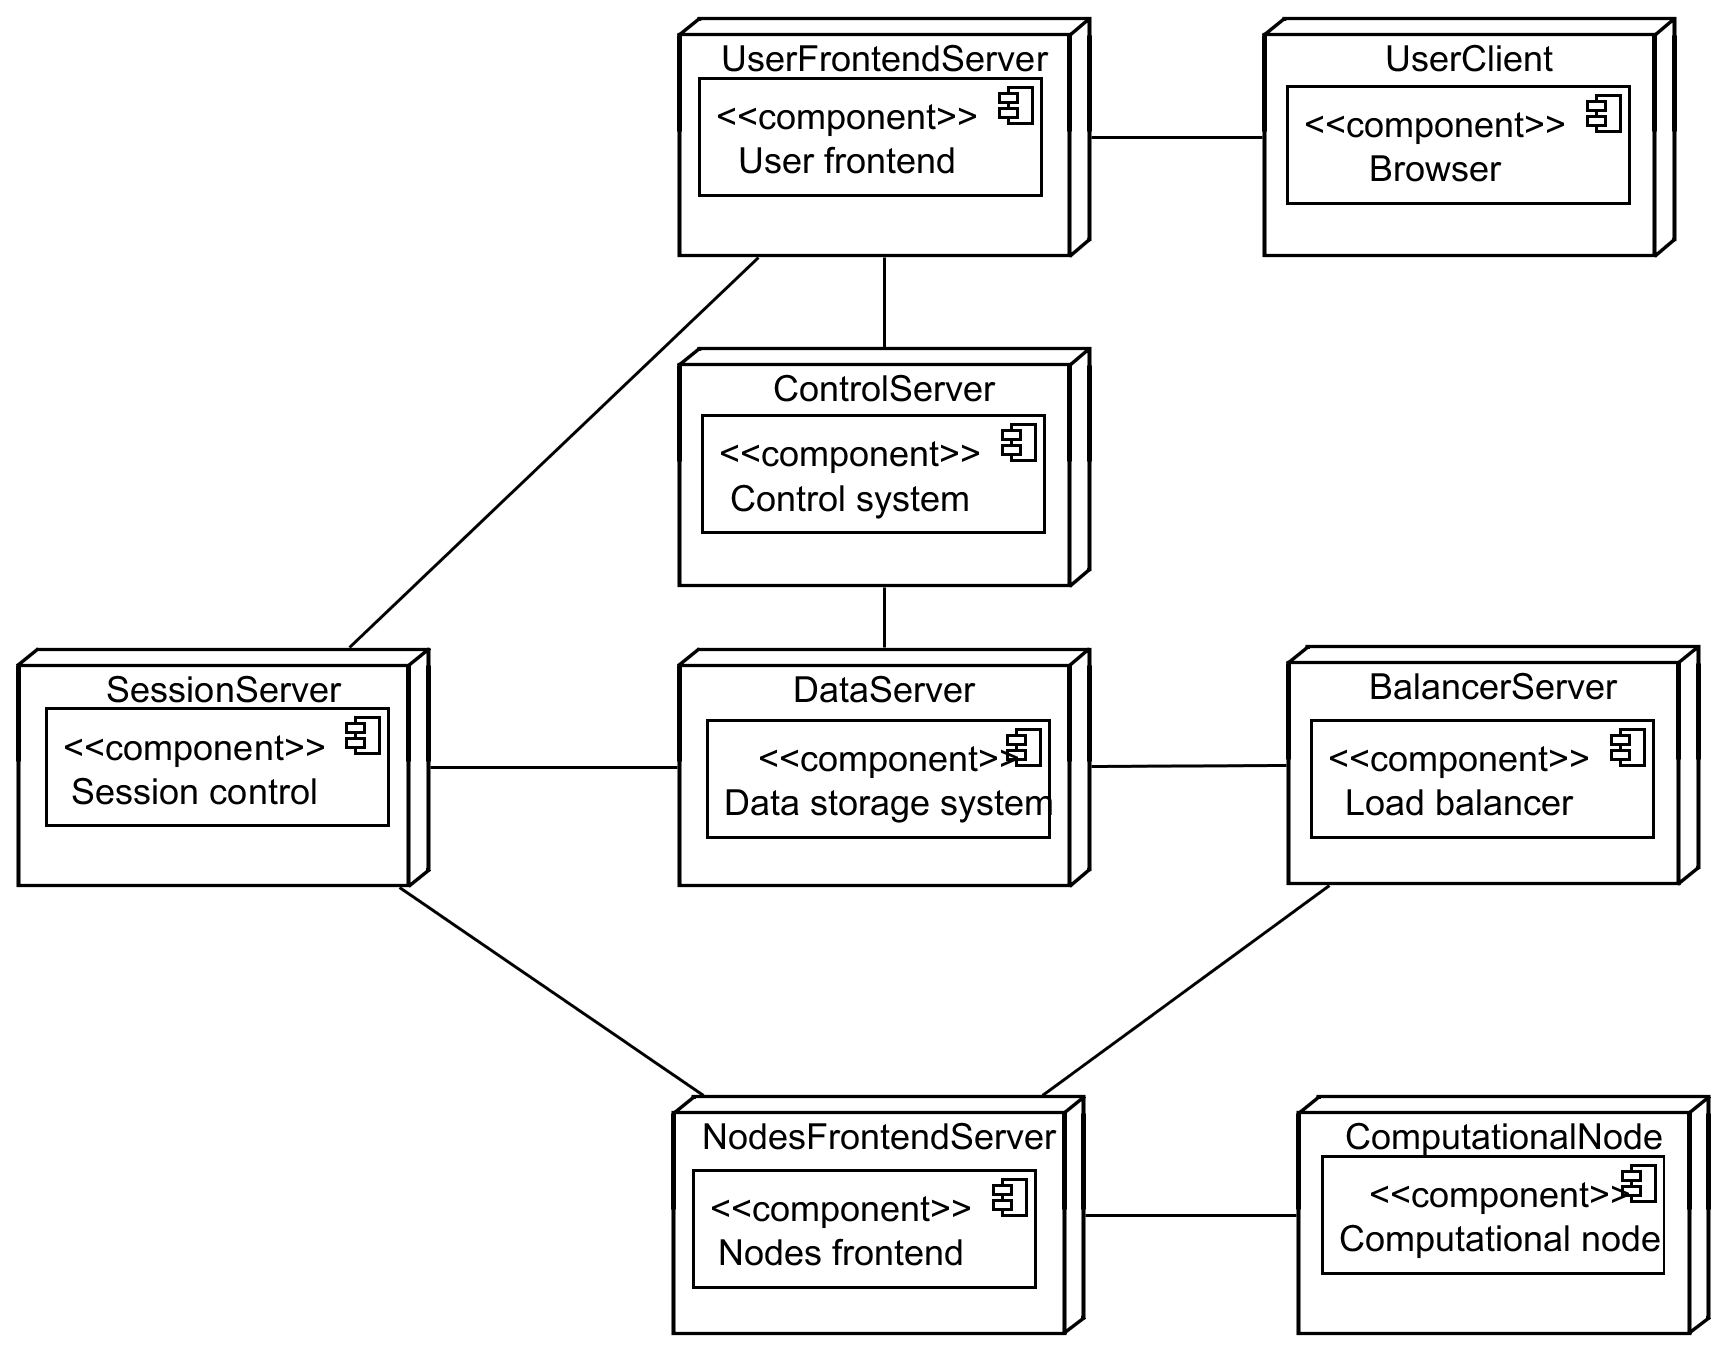
\includegraphics[width=\linewidth]{diagrams/common/deployment}
  \caption{Диаграмма развёртывания комплекса}
  \label{fig:depl-common}
\end{figure}

\subsection{Система мониторинга}
Задача данной подсистемы -- отслеживание топологии сети.
Все узлы комплекса должны оповещать СМ о своём статусе работы, 
и любой узел может получить от комплекса список активных в данный момент узлов.
Данная система является полностью пассивной.

Невозможность любой другой подсистемы связаться с системой мониторинга рассматривается
как ошибка сети, нарушающая нормальное функционирование комплекса.

\subsubsection{Пассивная часть}
Исходя из требований к СМ и с учётом REST-методик, она должна предоставлять следующее API:

\begin{itemize}
  \item
  \begin{description}
    \item[Ресурс:] \url{/services}
    \item[Метод:] GET
    \item[Результат:] список активных сервисов
  \end{description}
  \item
  \begin{description}
    \item[Ресурс:] \url{/services/type}
    \item[Метод:] GET
    \item[Результат:] список активных сервисов такого типа
  \end{description}
  \item
  \begin{description}
    \item[Ресурс:] \url{/services/type}
    \item[Метод:] POST
    \item[Параметры:] port, state?
    \item[Результат:] сообщение об успешной регистрации сервиса и распознанный адрес сервиса
    \item[Ошибки:] отсутствует параметр 'port': HTTP 422
  \end{description}
  \item
  \begin{description}
    \item[Ресурс:] \url{/services/type/address}
    \item[Метод:] GET
    \item[Результат:] статусное сообщение выбранного сервиса, аннотированное временем создания
    \item[Ошибки:] сервис не найден: HTTP 404
  \end{description}
  \item
  \begin{description}
    \item[Ресурс:] \url{/services/type/address}
    \item[Метод:] PUT
    \item[Параметры:] state?
    \item[Результат:] сообщение об успешном обновлении статусного сообщения
  \end{description}
\end{itemize}

Коллекция верхнего уровня \url{/services} имеет словарь JSON-формата, приведённого на примере в листинге~\ref{lst:json-beacon}. Запросы к коллекциям более глубокого уровня \url{/services/type} и \url{/services/type/address} отображаются в подсловари root[type] и root[type][address] словаря верхнего уровня, соответственно.

\begin{lstlisting}[float={},language=Java,caption={Пример JSON-представления коллекции верхнего уровня сервиса мониторинга},label=lst:json-beacon]
{
  "type1": {
    "ipaddr1:port1": {
      "state": "message1", 		// arbitrary string
      "lastbeat": "datetime1"	// ex. "2015-05-25 01:46:35.857670"
    },
    "ipaddr2:port2": {
      "state": "message2",
      "lastbeat": "datetime2"
    }
  },
  "type2": {
    "ipaddr3:port3": {
      "state": "message3",
      "lastbeat": "datetime3"
    }
  }
}
\end{lstlisting}

\subsection{Фронтэнд пользователей}
Задача данной подсистемы -- проверки безопасности и перенаправление запросов от пользователей к системе управления, а также отрисовка веб-интерфейса.

\subsubsection{Активная часть}
\begin{itemize}
  \item В ходе конфигурирования данной системы необходимо в ручном порядке указать адрес системы мониторинга.
  \item ФП должен зарегистрироваться на СМ и оповещать её о своём состоянии с некоторой периодичностью.
  \item В ходе работы ФП должен получать со стороны СМ информацию о текущем адресе СУ и СУС.
\end{itemize}

\subsubsection{Пассивная часть}
Исходя из требований к ФП, он должен предоставлять следующий функционал:

\begin{itemize}
  \item регистрация пользователя
  \item авторизация пользователя
  \item просмотр списка существующих в системе черт
  \item постановка задачи с передачей в систему описания задачи, содержащего:
  \subitem файл со списком черт задачи
  \subitem все необходимые для запуска задачи файлы
  \subitem в зависимости от платформы, либо файл run.bat, либо файл run.sh, осуществляющий запуск программы
  \subitem список выходных файлов задачи в файле output.txt
  \item просмотр статусов поставленных задач
  \item для выполненных задач -- просмотр результатов выполнения
  \item удаление задач
\end{itemize}

На файлы, составляющие описание задачи, накладываются следующие ограничения:

\begin{itemize}
  \item Все файлы, кроме файла traits.txt, должны содержаться в zip-архиве.
  \item Файл traits.txt должен содержать набор строк в кодировке UTF-8.
  В каждой строке должна быть записана очередная черта задачи.
  Черта задачи состоит из имени черты и версии черты, разделёнными символом табуляции
  Файл может заканчиваться пустой строкой.
  Пример корректного файла дан в листинге~\ref{lst:task-traits}.
  \item Файл output.txt должен содержать набор строк в кодировке UTF-8.
  В каждой строке должен быть записан путь к одному из выходных файлов.
  Началом пути считается корень архива.
  Файл может заканчиваться пустой строкой.
  Пример корректного файла дан в листинге~\ref{lst:task-output}.
  \item Файл run.bat / run.sh должен содержать инструкции по запуску задачи и корректно исполняться на вычислительном узле, удовлетворяющем требованиям, описанных чертами задачи.
  Именно этот файл будет запущен вычислительным узлом для начала расчётов.
  По завершении выполнения задачи она должна закрыть все созданные окна и уничтожить все порождённые процессы.
\end{itemize}

\begin{lstlisting}[float={},language={},caption={Пример корректного файла со списком черт задачи},label=lst:task-traits]
root_folder_file.txt
directory/subdirectory_file.extension

\end{lstlisting}

\begin{lstlisting}[float={},language={},caption={Пример корректного файла со списком выходных файлов},label=lst:task-output]
root_folder_file.txt
directory/subdirectory_file.extension

\end{lstlisting}

\subsection{Фронтэнд вычислительных узлов}
Задача данной подсистемы -- перенаправление запросов от вычислительных узлов на балансировщик нагрузки.

\subsubsection{Активная часть}
\begin{itemize}
  \item В ходе конфигурирования данной системы необходимо в ручном порядке указать адрес системы мониторинга.
  \item ФВУ должен зарегистрироваться на СМ и оповещать её о своём состоянии с некоторой периодичностью.
  \item В ходе работы ФВУ должен получать со стороны СМ информацию о текущем адресе СБН.
\end{itemize}

\subsubsection{Пассивная часть}
Исходя из требований к ФВУ и с учётом REST-методик, он должен предоставлять следующее API:

\begin{itemize}
  \item
  \begin{description}
    \item[Ресурс:] \url{/nodes}
    \item[Метод:] POST
    \item[Параметры:] список черт вычислительного узла
    \item[Результат:] сообщение об успешной регистрации узла и назначенный идентификатор
  \end{description}
  \item
  \begin{description}
    \item[Ресурс:] \url{/nodes/nodeid}
    \item[Метод:] PUT
    \item[Параметры:] состояние расчёта
    \item[Результат:] сообщение об успешном обновлении статуса
  \end{description}
  \item
  \begin{description}
    \item[Ресурс:] \url{/tasks/newtask}
    \item[Метод:] GET
    \item[Параметры:] идентификатор вычислительного узла
    \item[Результат:] пакет данных, описывающих задачу
    \item[Ошибки:] подходящих задач нет: HTTP 404; идентификатор не распознан либо отсутствует: HTTP 422
  \end{description}
  \item
  \begin{description}
    \item[Ресурс:] \url{/tasks/taskid}
    \item[Метод:] POST
    \item[Параметры:] идентификатор вычислительного узла, результат выполнения задачи
    \item[Результат:] сообщение об успешном приёме результата
    \item[Ошибки:] ошибка идентификатора узла, формата задачи либо идентификатора задачи: HTTP 422
  \end{description}
\end{itemize}

Методы API POST \url{/nodes}, PUT \url{/nodes/nodeid}, GET \url{/tasks/newtask} и POST \url{/tasks/taskid} соответствуют прецедентам "регистрация", "запрос новой задачи", "отчёт о выполнении задачи" и "завершение выполнения задачи" соответственно.

Диаграммы последовательности действий при выполнении прецедентов "регистрация", "запрос новой задачи" и "завершение выполнения задачи" приведены на рис.~\ref{fig:seq-reg}, \ref{fig:seq-req}~и~\ref{fig:seq-sub}.

\begin{figure}
  \centering
  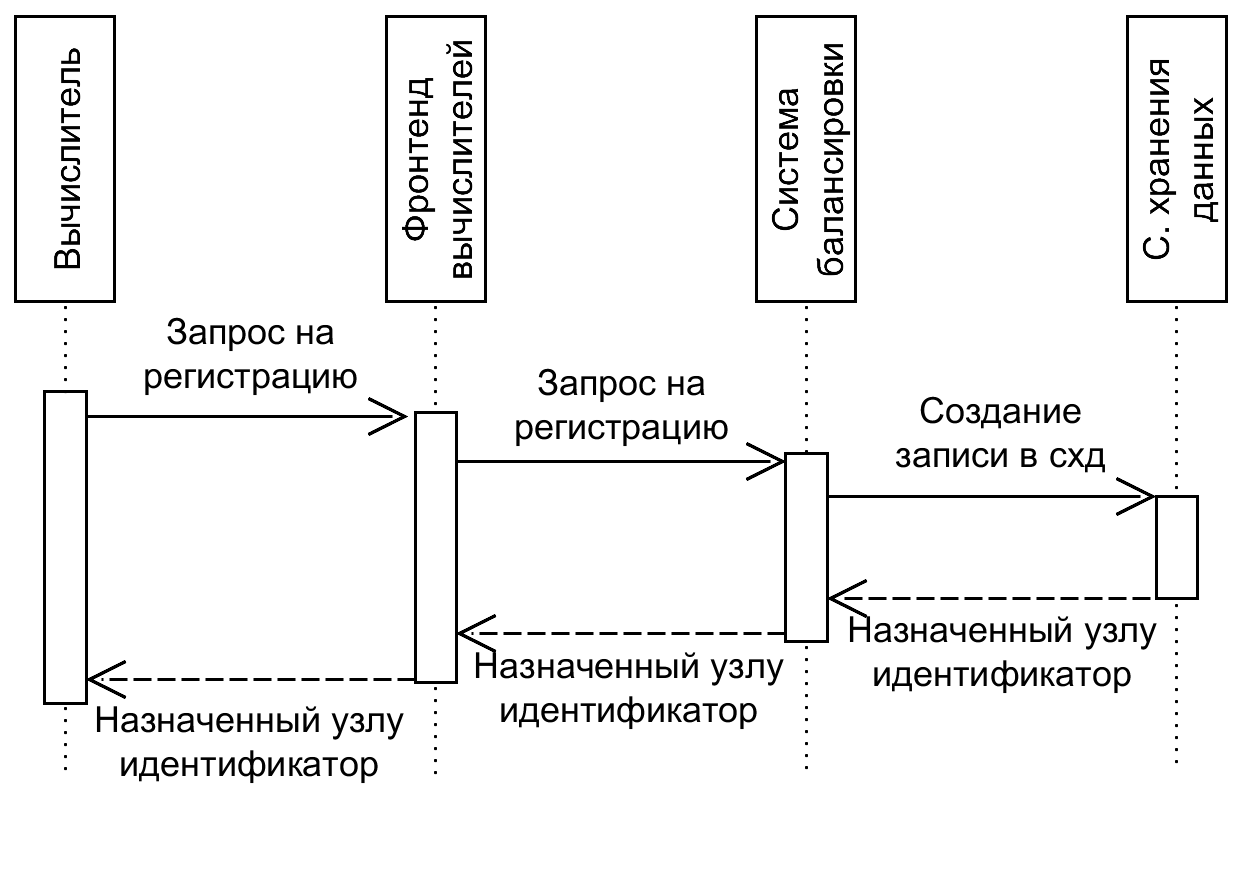
\includegraphics[width=.7\linewidth]{diagrams/frontnode/seq-register}
  \caption{Диаграмма последовательности действий прецедента "регистрация" ФВУ}
  \label{fig:seq-reg}
\end{figure}

\begin{figure}
  \centering
  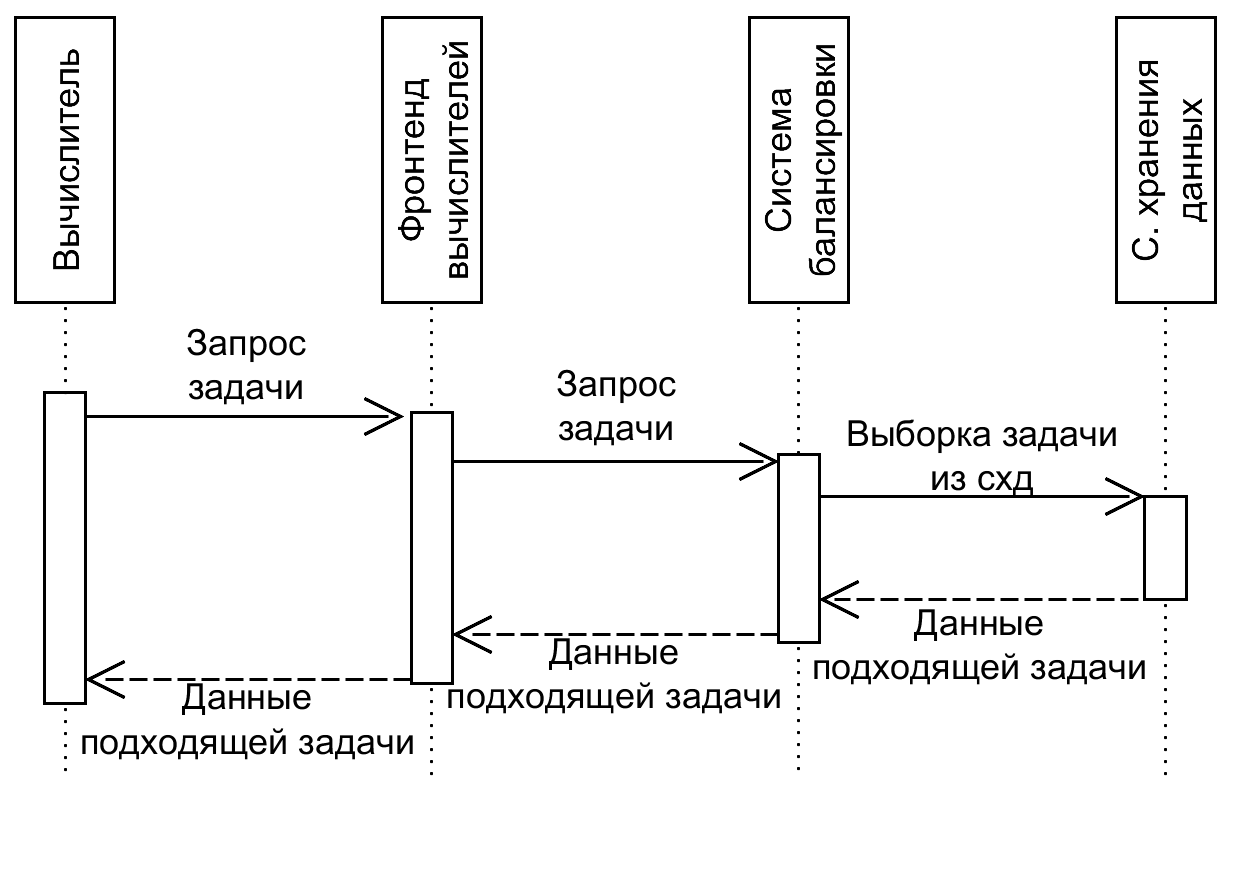
\includegraphics[width=.7\linewidth]{diagrams/frontnode/seq-request}
  \caption{Диаграмма последовательности действий прецедента "запрос новой задачи" ФВУ}
  \label{fig:seq-req}
\end{figure}

\begin{figure}
  \centering
  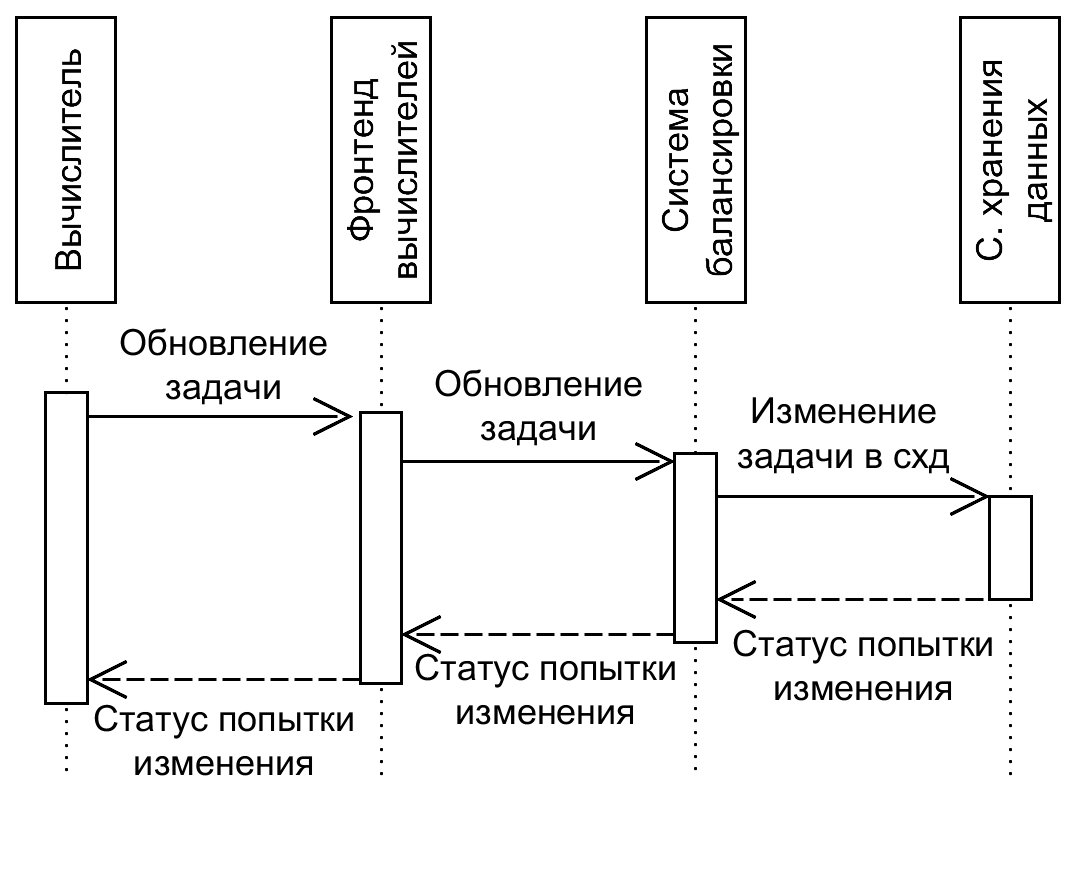
\includegraphics[width=.7\linewidth]{diagrams/frontnode/seq-submit}
  \caption{Диаграмма последовательности действий прецедента "завершение выполнения задачи" ФВУ}
  \label{fig:seq-sub}
\end{figure}

\subsection{Система управления сессией}
Задача данной подсистемы -- регистрация, авторизация и аутентификация пользователей в сети.

\subsubsection{Активная часть}
\begin{itemize}
  \item В ходе конфигурирования данной системы необходимо в ручном порядке указать адрес системы мониторинга.
  \item СУС должна зарегистрироваться на СМ и оповещать её о своём состоянии с некоторой периодичностью.
\end{itemize}

\subsubsection{Пассивная часть}
Исходя из требований к СУС и с учётом REST-методик, она должна предоставлять следующее API:

\begin{itemize}
  \item
  \begin{description}
    \item[Ресурс:] \url{/users}
    \item[Метод:] POST
    \item[Параметры:] желаемая пара логин / пароль (возможно, хешированный)
    \item[Результат:] сообщение об успешной регистрации пользователя
    \item[Ошибки:] пользователь с таким именем уже зарегистрирован: HTTP 403
  \end{description}
  \item
  \begin{description}
    \item[Ресурс:] \url{/users/username}
    \item[Метод:] GET
    \item[Параметры:] пароль (возможно, хешированный)
    \item[Результат:] сгенерированный ключ доступа
    \item[Ошибки:] некорректная пара логин / пароль: HTTP 403
  \end{description}
  \item
  \begin{description}
    \item[Ресурс:] \url{/validate}
    \item[Метод:] GET
    \item[Параметры:] ключ доступа
    \item[Результат:] сообщение об успешной проверке ключа
    \item[Ошибки:] некорректный ключ: HTTP 401
  \end{description}
\end{itemize}

\subsection{Система управления}
Задача данной системы -- предоставление API, позволяющего интерфейсной части (фронтэнду вычислительных узлов) осуществлять взаимодействие пользователя с комплексом.

\subsubsection{Активная часть}
\begin{itemize}
  \item В ходе конфигурирования данной системы необходимо в ручном порядке указать адрес системы мониторинга.
  \item СУ должна зарегистрироваться на СМ и оповещать её о своём состоянии с некоторой периодичностью.
  \item В ходе работы СУ должна получать со стороны СМ информацию о текущем адресе СХД.
\end{itemize}

\subsubsection{Пассивная часть}
Исходя из требований к СУ и с учётом REST-методик, она должна предоставлять следующее API:

\begin{itemize}
  \item
  \begin{description}
    \item[Ресурс:] \url{/foo}
    \item[Метод:] BAR
    \item[Параметры:] lorem
    \item[Результат:] ipsum
    \item[Ошибки:] dolor
  \end{description}
\end{itemize}

\subsection{Система хранения данных}
Задача данной системы -- хранение данных о задачах, вычислительных узлах и их чертах, а также предоставление API по доступу к этим данным.

Связи между разными типами хранимых данных предоставлены в виде ER-диаграммы на рис.~\ref{fig:db-er}.

\begin{figure}[h!]
  \centering
  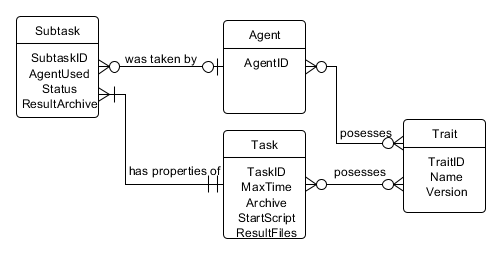
\includegraphics[width=.9\linewidth]{diagrams/db/er}
  \caption{ER-диаграмма сущностей, хранимых в СХД}
  \label{fig:db-er}
\end{figure}

\subsubsection{Активная часть}
\begin{itemize}
  \item В ходе конфигурирования данной системы необходимо в ручном порядке указать адрес системы мониторинга.
  \item СХД должна зарегистрироваться на СМ и оповещать её о своём состоянии с некоторой периодичностью.
\end{itemize}

\subsubsection{Пассивная часть}
Исходя из требований к СХД и с учётом REST-методик, она должна предоставлять следующее API:
\\
Условные обозначения:
\begin{itemize}
  \item table -- имя таблицы в БД
  \item PKC -- поле, являющееся (целочисленным) первичным ключом
  \item GFSbAI -- get\_free\_subtask\_by\_agent\_id
  \item object -- \{field: value, ...\}, JSON-представление табличного объекта
  \item object <table> -- JSON-предтавление объекта определенной таблицы <table>
  \item value <name> -- значение, передаваемое любым возможным способом
  \item arrfilter object -- \{field: list value, ...\}
  \item filter object -- object, содержащий не более чем полный набор полей табличного объекта
  \item filter put object -- \{field:value, ..., ``changes'': filter object\}
  \item list object -- список объектов
  \item int -- целое число
\end{itemize}

%\begin{table}[h!]
\begin{longtabu} to \textwidth {*{4}{|c}|X|}
\hline
Адрес & Метод & Ввод & Код & Вывод \\
\hline
\multirow{5}{*}{/table}                & \multirow{3}{*}{POST}    & \multirow{3}{*}{object} 
                                                                      & 200 & empty \\
                                                                      \cline{4-5}
                                       &                          &   & 400 & error: Incorrect / insufficient input \\
                                                                      \cline{4-5}
                                       &                          &   & 500 & error: Postgres error or ``entry already exists'' \\
                                       \cline{2-5}
                                       & \multirow{2}{*}{GET}     & \multirow{2}{*}{--}     
                                                                      & 200 & \{``result'': list object\} \\
                                                                      \cline{4-5}
                                       &                          &   & 404 & error: Not found \\
\hline
\multirow{6}{*}{/table/filter}         & \multirow{2}{*}{GET}     & \multirow{2}{*}{filter object} 
                                                                      & 200 & \{``result'': list object\} \\
                                                                      \cline{4-5}
                                       &                          &   & 400 & error: Incorrect fields/values specified \\
                                       \cline{2-5}
                                       & \multirow{2}{*}{PUT}     & \multirow{2}{*}{filter put object} 
                                                                      & 200 & \{``count'': int\}\\
                                                                      \cline{4-5}
                                       &                          &   & 400 & error: Incorrect fields/values specified \\
                                       \cline{2-5}
                                       & \multirow{2}{*}{DELETE}  & \multirow{2}{*}{filter object}
                                                                      & 200 & \{``count'': int\}\\
                                                                      \cline{4-5}
                                       &                          &   & 400 & error: Incorrect fields/values specified \\
\hline
\multirow{2}{*}{/table/arrayfilter}    & \multirow{2}{*}{GET}     & \multirow{2}{*}{arrayfilter object} 
                                                                      & 200 & \{``result'': list object\} \\
                                                                      \cline{4-5}
                                       &                          &   & 400 & error: Incorrect fields/values specified \\
%                                       \cline{2-5}
%                                       & \multirow{2}{*}{PUT}     & \multirow{2}{*}{filter put object} 
%                                                                      & 200 & \{``count'': int\}\\
%                                                                      \cline{4-5}
%                                       &                          &   & 400 & error: Incorrect fields/values specified \\
%                                       \cline{2-5}
%                                       & \multirow{2}{*}{DELETE}  & \multirow{2}{*}{filter object}
%                                                                      & 200 & \{``count'': int\}\\
%                                                                      \cline{4-5}
%                                       &                          &   & 400 & error: Incorrect fields/values specified \\
\hline
\multirow{9}{*}{/table/PKC/value}      & \multirow{3}{*}{GET}  & \multirow{2}{*}{object} 
                                                                      & 200 & object \\
                                                                      \cline{4-5}
                                       &                          &   & 400 & error: Incorrect fields/values specified \\
                                                                      \cline{4-5}
                                       &                          &   & 404 & error: Not found \\
                                       \cline{2-5}
                                       & \multirow{3}{*}{PUT}     & \multirow{2}{*}{object} 
                                                                      & 200 & object \\
                                                                      \cline{4-5}
                                       &                          &   & 400 & error: Incorrect fields/values specified \\
                                                                      \cline{4-5}
                                       &                          &   & 404 & error: Not found \\
                                       \cline{2-5}
                                       & \multirow{3}{*}{DELETE}  & \multirow{2}{*}{object}
                                                                      & 200 & object \\
                                                                      \cline{4-5}
                                       &                          &   & 400 & error: Incorrect fields/values specified \\
                                                                      \cline{4-5}
                                       &                          &   & 404 & error: Not found \\
\hline
\multirow{2}{*}{/custom/GFSbAI}        & \multirow{2}{*}{GET}     & \multirow{2}{*}{value agent\_id} 
                                                                      & 200 & object subtask \\
                                                                      \cline{4-5}
                                       &                          &   & 400 & error: Incorrect value specified \\
\hline
\end{longtabu}
%\end{table}
Кроме указанных кодов ошибок, также все запросы могут вернуть в ответ ошибки со следующими кодами:
\begin{itemize}
  \item 408 -- Таймаут попытки доступа к некоторому шарду;
  \item 456 -- Получены различные ошибки от шардов при выполнении запроса. Эта ошибка является следствием нарушения согласованности данных.
\end{itemize}

\subsection{Система балансировки нагрузки}
--- собственно отвечает за координацию задач. имеет всё апи фронтенда вычислительных узлов (который просто редиректит запросы к ней), плюс некоторое апи по которому её опрашивают другие узлы комплекса.
%Задача данной системы -- предоставление API, управление и координация, прецеденты?

\subsubsection{Активная часть}
\begin{itemize}
  \item В ходе конфигурирования данной системы необходимо в ручном порядке указать адрес системы мониторинга.
  \item СБН должна зарегистрироваться на СМ и оповещать её о своём состоянии с некоторой периодичностью.
  \item В ходе работы СБН должна получать со стороны СМ информацию о текущем адресе СХД.
\end{itemize}

\subsubsection{Пассивная часть}
Исходя из требований к СБН и с учётом REST-методик, она должна предоставлять API, идентичное предоставляемому фронтэндом вычислительных узлов.

\subsection{Система вычисления}
Данная система представлена набором вычислительных узлов с установленным на них специальным ПО, 
осуществляющем взаимодействие с остальными сервисами системы и управление ходом выполнения задачи.

\subsubsection{Активная часть}
В ходе конфигурирования данной системы необходимо в ручном порядке указать адрес фронтэнда вычислительных узлов.

ПО, обеспечивающее функционирование системы, должно удовлетворять следующим требованиям:
\begin{itemize}
  \item До подключения к серверу балансировки приложение должно предоставлять возможность формирования списка черт, характеризующих АО и ПО вычислительного узла
  \item После подключения к балансировщику (через фронтэнд вычислительных узлов), с определённой периодичностью вычислительный узел должен опрашивать комплекс на предмет наличия доступных задач
  \item По получении задачи, вычислительный узел должен с определённой периодичностью оповещать балансировщик о ходе выполнения задачи
  \item По завершении выполнения задачи, вычислительный узел должен передать балансировщику сведения о результате выполнения задачи
\end{itemize}

Диаграмма состояний ПО вычислительного узла, иллюстрирующая приведённые выше соображения, приведена на рис.~\ref{fig:node-state}.

\begin{figure}
  \centering
  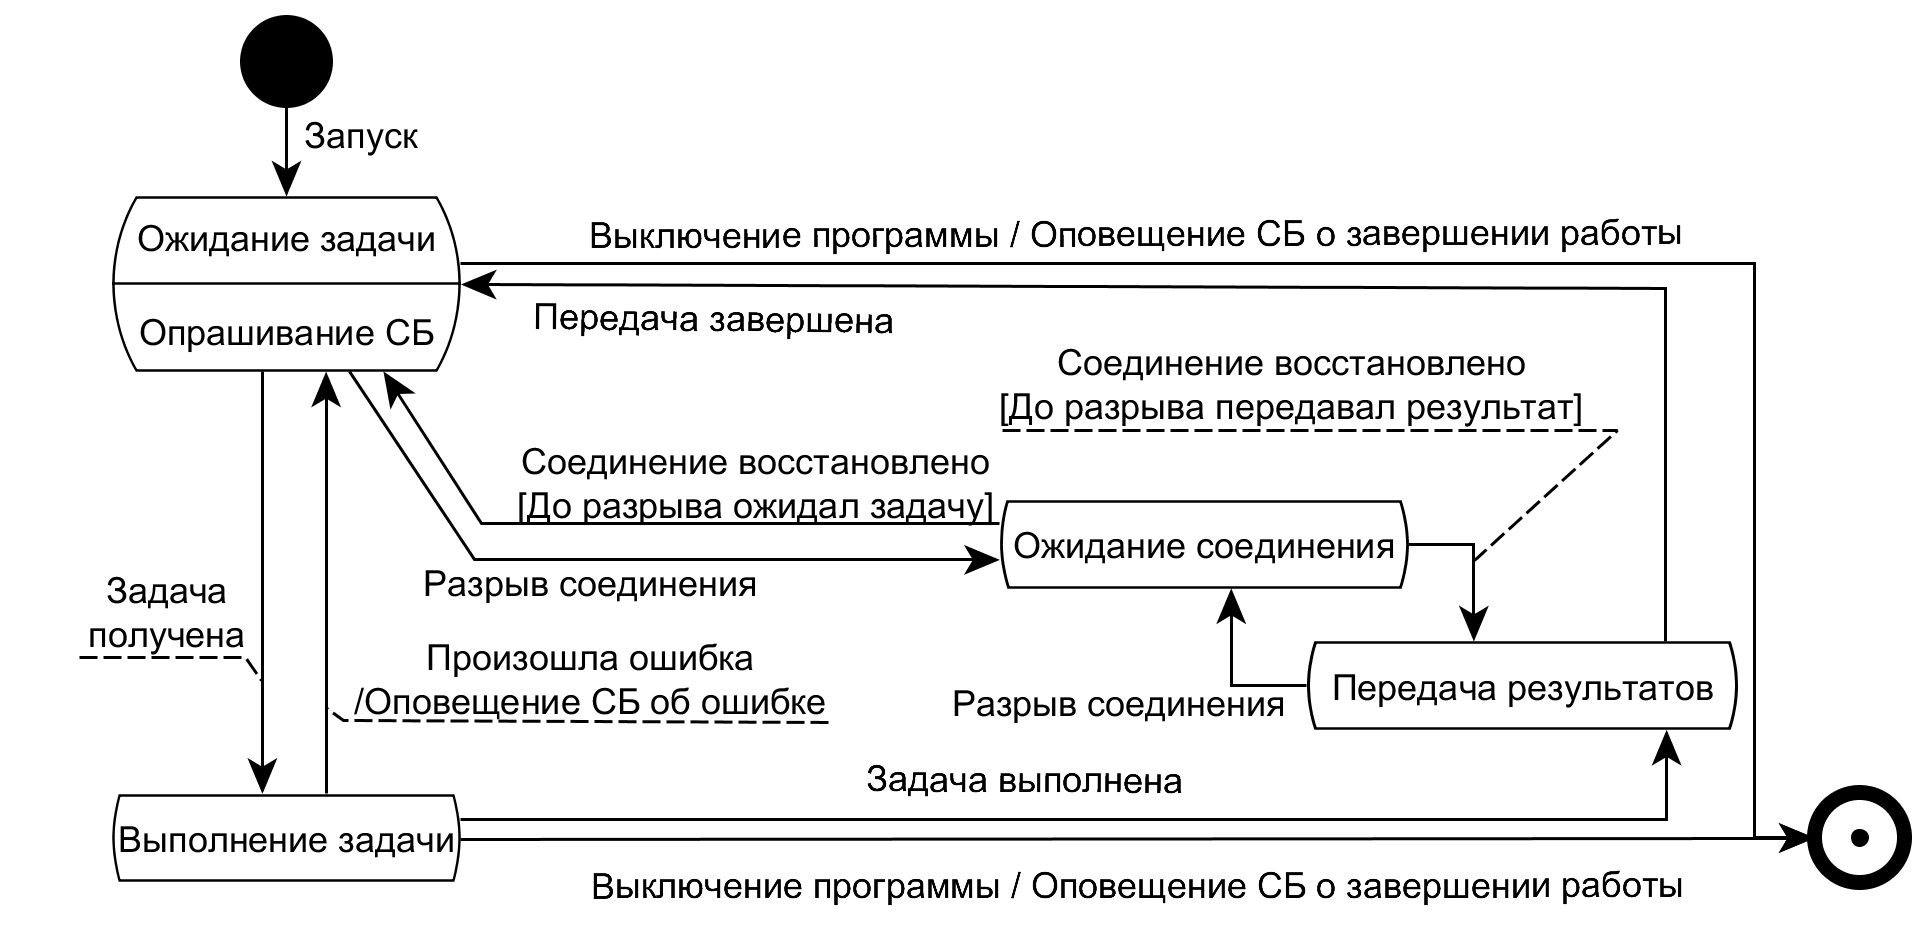
\includegraphics[width=\linewidth]{diagrams/compnode/state}
  \caption{Диаграмма состояний ВУ}
  \label{fig:node-state}
\end{figure}

\subsection{Вывод}

\clearpage
\section{Технологический раздел}
\subsection{Введение}
В данном разделе производится выбор языка программирования и сопутствующих программных средств. 
Описываются основные моменты программной реализации и описывается методика тестирования.

\subsection{Выбор языка программирования}

\subsection{Выбор программных средств}
перечень средств:
python
  flask
  jsonpickle
  

\subsection{Система мониторинга}
\subsubsection{Реализация}
Система была реализована с помощью python-фреймворка flask.
Для сериализации данных в json-формат и обратно была использована библиотека jsonpickle.
Исходный код системы приведён в приложении~[необходимо разобраться с автонумерацией приложений].

\subsubsection{Тестирование}
В ходе юнит-тестирования проверялись следующие сценарии:

\begin{itemize}
  \item доступ к отсутствующему элементу через ресурсы \url{/services}, \url{/services/type} и \url{/services/type/address};
  \item попытка создания записи по ресурсу \url{/services/test} без указания порта;
  \item попытка создания записи по ресурсу \url{/services/test};
  \item выборка всех активных сервисов по ресурсу \url{/services};
  \item выборка активных сервисов роли test по ресурсу \url{/services/test};
  \item изменение статусного сообщения сервиса по ресурсу \url{/services/test/address};
  \item проверка удаления сервиса из списка активных после определённого времени неактивности.
\end{itemize}

Тест был выполнен на языке Python.
%Исходный код теста приведён в листинге в приложении такомто
Выход теста приведён в листинге~\ref{lst:test-beacon-testout}.
Соответствующие сообщения сервера приведены в листинге~\ref{lst:test-beacon-servout}.

\lstinputlisting[float={},language={},caption={Выход юнит-теста системы мониторинга},label=lst:test-beacon-testout]{tests/beacon/tester.txt}

\lstinputlisting[float={},language={},caption={Сообщения системы мониторинга в ходе юнит-теста},label=lst:test-beacon-servout]{tests/beacon/service.txt}

\subsection{Фронтэнд пользователей}
\subsubsection{Реализация}

\subsubsection{Тестирование}

\subsection{Фронтэнд вычислительных узлов}
\subsubsection{Реализация}

\subsubsection{Тестирование}
\subsection{Система управления сессией}
\subsubsection{Реализация}

\subsubsection{Тестирование}

\subsection{Система управления}
\subsubsection{Реализация}

\subsubsection{Тестирование}

\subsection{Система хранения данных}
\subsubsection{Реализация}

\subsubsection{Тестирование}

\subsection{Система балансировки нагрузки}
\subsubsection{Реализация}

\subsubsection{Тестирование}

\subsection{Система вычисления}
\subsubsection{Реализация}

\subsubsection{Тестирование}

\subsection{Вывод}

\clearpage
\section{Заключение}

\section{Список литературы}
%\printbibliography[heading=none]

%разобраться с автонумерацией приложений
%\section*{\titleline[r]{Приложение 1}} \addcontentsline{toc}{section}{Приложение 1}
%\subsection*{Конфигурационный файл Alex}
%\lstinputlisting[float={},language=Python,caption={Исходный код юнит-теста системы мониторинга},label=lst:test-beacon]{tests/beacon/service}
%\clearpage


\end{document}